\documentclass[11pt]{article}
\textwidth 15.9cm
\textheight 23. cm
\addtolength{\oddsidemargin}{-11.5mm}
\addtolength{\evensidemargin}{-11.5mm}
\addtolength{\topmargin}{-19.0mm}

%\usepackage{amsmath}
\usepackage[T1]{fontenc}
\usepackage[ansinew]{inputenc}
\usepackage[bbgreekl]{mathbbol}
\usepackage{amsmath,amssymb}
\usepackage{graphicx}
\usepackage[colorlinks=true,urlcolor=cyan]{hyperref}%,linkcolor=green]{hyperref}
\usepackage{url}
\usepackage[numbers,square]{natbib}
\usepackage{multirow}
\usepackage{tikz}
\usepackage{tikz-cd}
\usetikzlibrary{arrows,matrix}
\usepackage{bbm}
\usepackage{authblk}
\usepackage{subcaption}
\usepackage{xstring}
\usepackage{xparse}
\usepackage{comment}
\renewcommand{\Affilfont}{\footnotesize}

%\renewcommand{\Authfont}{\normalsize}
\usepackage{mdframed}
\newenvironment{important}[1][]{%
   \begin{mdframed}[%
      backgroundcolor={red!15}, hidealllines=true,
      skipabove=0.7\baselineskip, skipbelow=0.7\baselineskip,
      splitbottomskip=2pt, splittopskip=4pt, #1]%
   \makebox[0pt]{% ignore the withd of !
      \smash{% ignor the height of !
         \fontsize{32pt}{32pt}\selectfont% make the ! bigger
         \hspace*{-19pt}% move ! to the left
         \raisebox{-2pt}{% move ! up a little
            {\color{red!70!black}\sffamily\bfseries !}% type the bold red !
         }%
      }%
   }%
}{\end{mdframed}}
%\usepackage{algpseudocode}

\usepackage{listings}
\usepackage{xcolor}
\usepackage[most]{tcolorbox}
\definecolor{lightergray}{gray}{0.95}
\definecolor{macrocolor}{RGB}{255,145,0}
\definecolor{warningred}{RGB}{255,145,145}
\newtcolorbox{customWarning}{colback=warningred,grow to right by=-10mm,grow to left by=-10mm, boxrule=0pt,boxsep=0pt,breakable}
\usepackage{expl3}

\ExplSyntaxOn

% compile the expression
\regex_new:N \l_CPP_uppercase_regex
%\regex_set:Nn \l_CPP_uppercase_regex { ^ [A-Z\_]+ $ } % somehow, "_" char cannot be escaped
\regex_set:Nn \l_CPP_uppercase_regex { ^ [^\w\s]?([A-Z]+[^\w\s]?)+ $ } % Replacement hack.

\regex_new:N \l_completely_unused_regex       % Editor thinks the entire rest of the doc is
\regex_set:Nn \l_completely_unused_regex {^$} % in math mode unless we provide a second $.

% a variant that expands the input fully
\cs_generate_variant:Nn \regex_match:NnTF {NV}

\NewDocumentCommand \ifuppercase { m m }
{
    % expand to actual underscore
    \cs_set_eq:Nc \__CPP_uppercase_um { lst@um_ }
    \tl_set:cn { lst@um_ } { _ }
    % match the current token
    \regex_match:NVTF \l_CPP_uppercase_regex {\the\use:c{lst@token}} {#1} {#2}
    % reset
    \cs_set_eq:cN { lst@um_ } \__CPP_uppercase_um
}

\ExplSyntaxOff



\lstset{language=C++,
        morekeywords={constexpr},
        keywordstyle=\color{blue}\bfseries,
        alsoletter={_},
        basicstyle=\ttfamily,
        columns=fullflexible,
        identifierstyle=\ifuppercase{\color{macrocolor}\bfseries}{},
        backgroundcolor=\color{lightergray}}

\usepackage{stmaryrd}
\usepackage{comment}
\usepackage{showlabels}
\usepackage{soul}
%\usepackage[dvipsnames]{xcolor}

\usetikzlibrary{calc,patterns,shapes.geometric}
\usetikzlibrary{arrows,shapes,positioning}
\usetikzlibrary{decorations.markings,decorations.pathmorphing,decorations.pathreplacing}
\usetikzlibrary{decorations.text,decorations.shapes}

%%%%%%%% MACROS
%% Macros for Gempic/Gempif papers
%
% legend for main math fonts:
%
% - vectors or vector-valued functions (with physical dimension > 1)
%   bold math font: prefix \b
%   \bE, \bB, \bLambda ...
%
% - arrays of stacked quantities (dim = numerical parameter)
%   bold sans-serif fonts: prefix \arr
%   \arrX, \arrE, \arrLambda ...
%
% - matrices & discrete operators between arrays
%   blackboard sans-serif: prefix \mat
%   \matM, \matJ ...
%
% - usual number sets
%   standard blackboard
%   \NN, \RR ...
%
% - functionals and some operators
%   caligraphic math: prefix \c
%   \cL, \cI ...


% \usepackage[bbgreekl]{mathbbol}
% \usepackage{amsmath,amssymb}
% \usepackage{amsthm}  % added on 9.9.2020 -- no conflicts?
% \usepackage{bm}
%\usepackage{bbm}
% \usepackage{upgreek}


\def\blankfirst{\phantom{V^0} }
\def\blanksecond{\phantom{ \{ } } %\hspace*{-5pt}}
\def\bbb{\phantom{\big|} }
\def\bBb{\phantom{\Big|} }

\def\mint{\int \mspace{-21.mu}\raise .8ex\hbox{\rotatebox{-80}{$|$}\,}}
\def\smint{\smallint \mspace{-13.mu}\raise -.1ex\hbox{\rotatebox{10}{--}}}

\DeclareMathOperator{\supp}{supp}
\DeclareMathOperator{\rank}{rank}
\providecommand{\bproofof}[1]{\bigskip\noindent{\em Proof of #1.}~}
\def\bproof{\bigskip\noindent{\em Proof.}~}
\def\eproof{\hfill$\square$\nl}

\def\beq{\begin{equation}}
\def\eeq{\end{equation}}

\def\bs{\boldsymbol}

\def\ds{\displaystyle}
\def\nl{\newline}
\def\noi{\noindent}  %\ni = reverse \in

\def\<{\langle}
\def\>{\rangle}

\def\ie{{\em i.e. }}
\def\eg{{\em e.g. }}
\def\inc{{\rm in }}
% need to be redefined for mathjax
\providecommand{\bm}{}
\renewcommand{\bm}[1]{\bs {\rm #1}}
\renewcommand{\mathbbm}[1]{\mathbb{#1}}

\def\h{\hat}
\def\wh{\widehat}
%\def\t{\tilde}
\renewcommand{\t}[1]{\tilde{#1}}
\def\wt{\widetilde}
\def\u{\underline}
\def\Chi{\raise .3ex \hbox{\large $\chi$}} %\def\vp{\varphi}

\newcommand{\ii}{\ensuremath{\mathrm{i}}}

\def\ex{{\rm ex}}

\def\rmd{\, {\rm d}} %for integrals
\def\dd{\, {\rm d}} %for integrals also

\def\tb{\hbox{$\|\kern -.09em |$}}
\def\bigtb{\hbox{$\big\|\kern -.09em \big|$}}
\def\Bigtb{\hbox{$\Big\|\kern -.09em \Big|$}}
\newcommand\eref[1]{(\ref{#1})}

\def\GL{\mathbb{GL}}
\def\GO{\mathbb{GO}}

% macros for particle coordinates and grid nodes (to be changed if needed)
%
%\def\px{\bx}  % particle x, old
%\def\pv{\bv}  % particle v, old
\def\px{\bX}  % particle x, new
\def\pv{\bV}  % particle v, new

\def\pz{\bZ}  % particle variation, new
\def\py{\bY}  % particle w (var v), new

\def\gx{\bx}  % grid x

% macro for testing fields
\newcommand{\test}[1]{\check{#1}}

% macro for subitemizing
\newcommand{\SubItem}[1]{
    {\setlength\itemindent{15pt} \item[-] #1}
}


% blackboard fonts (eg for number sets)
% \mathbbm, \mathbbmss or \mathbbmtt with \usepackage{bbm}
\def\AA{\mathbbm{A}}
\def\BB{\mathbbm{B}}
\def\CC{\mathbbm{C}}
\def\DD{\mathbbm{D}}
\def\EE{\mathbbm{E}}
\def\FF{\mathbbm{F}}
\def\GG{\mathbbm{G}}
\def\II{\mathbbm{I}}
\def\JJ{\mathbbm{J}}
\def\KK{\mathbbm{K}}
\def\MM{\mathbbm{M}}
\def\NN{\mathbbm{N}}
\def\PP{\mathbbm{P}}
\def\QQ{\mathbbm{Q}}
\def\RR{\mathbbm{R}}
\def\SS{\mathbbm{S}}
\def\TT{\mathbbm{T}}
\def\UU{\mathbbm{U}}
\def\VV{\mathbbm{V}}
\def\WW{\mathbbm{W}}
\def\XX{\mathbbm{X}}
\def\YY{\mathbbm{Y}}
\def\ZZ{\mathbbm{Z}}

% black-board sans serif
% \mathbb require \usepackage ??  [bbgreekl]{mathbbol} of {upgreek} ??
\newcommand{\mat}[1]{\mathbb{#1}}
\def\matd{\mathbb{d}}
\def\matr{\mathbb{r}}
\def\matA{\mathbb{A}}
\def\matB{\mathbb{B}}
\def\matC{\mathbb{C}}
\def\matD{\mathbb{D}}
\def\matE{\mathbb{E}}
\def\matF{\mathbb{F}}
\def\matG{\mathbb{G}}
\def\matH{\mathbb{H}}
\def\matI{\mathbb{I}}
\def\matJ{\mathbb{J}}
\def\matK{\mathbb{K}}
\def\matM{\mathbb{M}}
\def\matN{\mathbb{N}}
\def\matO{\mathbb{O}}
\def\matR{\mathbb{R}}
\def\matS{\mathbb{S}}
\def\matT{\mathbb{T}}
\def\matt{\mathbb{t}}
\def\matW{\mathbb{W}}
\def\matw{\mathbb{w}}
\def\matZ{\mathbb{Z}}
\def\matLambda{\mathbb{\Lambda}}

\newcommand{\tildemat}[1]{\tilde{\mathbb{#1}}}

\def\LaB{\mathbb{\Lambda}} %% ?? delete

% arrays of stacked quantities (dim = numerical parameter)
\newcommand{\arr}[1]{{\bm{\mathsf{#1}}}}
\newcommand\arre{{\bm{\mathsf{e}}}}
\newcommand\arrg{{\bm{\mathsf{g}}}}
\newcommand\arrA{{\bm{\mathsf{A}}}}
\newcommand\arrB{{\bm{\mathsf{B}}}}
\newcommand\arrH{{\bm{\mathsf{H}}}}
\newcommand\arrb{{\bm{\mathsf{b}}}}
\newcommand\arrD{{\bm{\mathsf{D}}}}
\newcommand\arrE{{\bm{\mathsf{E}}}}
\newcommand\arrG{{\bm{\mathsf{G}}}}
\newcommand\arrJ{{\bm{\mathsf{J}}}}
\newcommand\arrU{{\bm{\mathsf{U}}}}
\newcommand\arrV{{\bm{\mathsf{V}}}}
\newcommand\arrW{{\bm{\mathsf{W}}}}
\newcommand\arrX{{\bm{\mathsf{X}}}}
\newcommand\arrY{{\bm{\mathsf{Y}}}}
\newcommand\arrZ{{\bm{\mathsf{Z}}}}
\newcommand\arrLambda{{\bm{\mathsf{\Lambda}}}}
\newcommand\arrsigma{{\bm{\mathsf{\sigma}}}}

\newcommand{\tildearr}[1]{{\tilde{\bm{\mathsf{#1}}}}}

% \newcommand\sfC{{\sf c}}
% \newcommand\sfE{{\sf e}}
% \newcommand\sfF{{\sf f}}
%
\newcommand\ttc{{\texttt{c}}}
\newcommand\tte{{\texttt{e}}}
\newcommand\ttf{{\texttt{f}}}

\newcommand\sfk{{\sf k}}
\newcommand\sfu{{\sf u}}
\newcommand\sfv{{\sf v}}
\newcommand\sfx{{\sf x}}
\newcommand\sfz{{\sf z}}

\newcommand\sfA{{\sf A}}
\newcommand\sfF{{\sf F}}
\newcommand\sfG{{\sf G}}
\newcommand\sfH{{\sf H}}
\newcommand\sfU{{\sf U}}
\newcommand\sfV{{\sf V}}
\newcommand\sfX{{\sf X}}

\def\Vsp{V}

\def\cA{\mathcal{A}}
\def\cB{\mathcal{B}}
\def\cC{\mathcal{C}}
\def\cD{\mathcal{D}}
\def\cE{\mathcal{E}}
\def\cF{\mathcal{F}}
\def\cG{\mathcal{G}}
\def\cH{\mathcal{H}}
\def\cI{\mathcal{I}}
\def\cK{\mathcal{K}}
\def\cL{\mathcal{L}}
\def\cN{\mathcal{N}}
\def\cO{\mathcal{O}}
\def\cP{\mathcal{P}}
\def\cQ{\mathcal{Q}}
\def\cR{\mathcal{R}}
\def\cS{\mathcal{S}}
\def\cT{\mathcal{T}}
\def\cX{\mathcal{X}}
\def\cV{\mathcal{V}}
\def\cW{\mathcal{W}}

\newcommand{\tcR}{\tilde{\mathcal{R}}}

\usepackage{mathrsfs}
\def\scrc{\mathscr{c}}
\def\scre{\mathscr{e}}
\def\scrf{\mathscr{f}}
\def\scrC{\mathscr{C}}
\def\scrE{\mathscr{E}}
\def\scrF{\mathscr{F}}
\def\scrP{\mathscr{P}}
\def\scrV{\mathscr{V}}

\newcommand\bfa{\mathbf{a}}
\newcommand\bfe{\mathbf{e}}
\newcommand\bff{\mathbf{f}}
\newcommand\bfq{\mathbf{q}}
\newcommand\bfg{\mathbf{g}}
\newcommand\bfl{\mathbf{l}}
\newcommand\bfr{\mathbf{r}}
\newcommand\bfv{\mathbf{v}}
\newcommand\bfw{\mathbf{w}}
\newcommand\bfx{\mathbf{x}}
\newcommand\bfy{\mathbf{y}}
\newcommand\bfz{\mathbf{z}}

\newcommand\bfve{\mathbf{\ve}}

\newcommand\bfA{\mathbf{A}}
\newcommand\bfB{\mathbf{B}}
\newcommand\bfE{\mathbf{E}}
\newcommand\bfJ{\mathbf{J}}
\newcommand\bfK{\mathbf{K}}
\newcommand\bfS{\mathbf{S}}
\newcommand\bfU{\mathbf{U}}
\newcommand\bfV{\mathbf{V}}
\newcommand\bfW{\mathbf{W}}
\newcommand\bfX{\mathbf{X}}
\newcommand\bfY{\mathbf{Y}}
\newcommand\bfZ{\mathbf{Z}}

%\newcommand\x{\bx}
%\newcommand\hbx{{\hat \bx}}
\newcommand\uvec{{\be}}

\newcommand{\one}{\ensuremath{\mathbbm{1}}}

\def\bcP{ \boldsymbol{\mathcal{P}} }
\def\bcB{ \boldsymbol{\mathcal{B}} }

\def\Np{N_{\rm part}}

\def\Mf{\MM_{\rm f}}
\def\Mp{\MM_{\rm p}}
\def\Qp{\QQ_{\rm p}}

\def\ba{{\bs a}}
\def\bb{{\bs b}}
\def\bc{{\bs c}}
\def\be{{\bs e}}
\def\bj{{\bs j}}
\def\bk{{\bs k}}
\def\bsm{{\bs m}}
\def\bn{{\bs n}}
\def\bp{{\bs p}}
\def\bq{{\bs q}}
\def\br{{\bs r}}
\def\bu{{\bs u}}
\def\bv{{\bs v}}
\def\bw{{\bs w}}
\def\bx{{\bs x}}
\def\by{{\bs y}}
\def\bz{{\bs z}}

\def\bA{{\bs A}}
\def\bB{{\bs B}}
\def\bC{{\bs C}}
\def\bE{{\bs E}}
\def\bF{{\bs F}}
\def\bG{{\bs G}}
\def\bH{{\bs H}}
\def\bI{{\bs I}}
\def\bJ{{\bs J}}
\def\bK{{\bs K}}
\def\bL{{\bs L}}
\def\bM{{\bs M}}
\def\bN{{\bs N}}
\def\bP{{\bs P}}
\def\bQ{{\bs Q}}
\def\bR{{\bs R}}
\def\bS{{\bs S}}
\def\bV{{\bs V}}
\def\bW{{\bs W}}
\def\bX{{\bs X}}
\def\bY{{\bs Y}}
\def\bZ{{\bs Z}}

\def\obu{{\overline {\bs u}}}
\def\bpi{{\bs \pi}}
\def\bell{{\bs \ell}}
\def\btau{{\bs \tau}}
\def\bphi{{\bs \phi}}
\def\bvp{{\bs \vp}}
\def\bxi{{\bs \xi}}
\def\bpsi{{\bs \psi}}
\def\bsigma{{\bs \sigma}}
\def\bLambda{{\bs \Lambda}}
\def\bPi{{\bs \Pi}}
\def\bPhi{{\bs \Phi}}
\def\bnabla{{\bs \nabla}}

\def\u{\underline}

\def\uE{{\u \bE}}
\def\uB{{\u B}}
\def\urho{{\u \rho}}
\def\uJ{{\u \bJ}}

\newcommand{\iph}{{i+\frac12}}
\newcommand{\jph}{{j+\frac12}}
\newcommand{\kph}{{k+\frac12}}
\newcommand{\imh}{{i-\frac12}}
\newcommand{\jmh}{{j-\frac12}}
\newcommand{\kmh}{{k-\frac12}}

%\newcommand{\bu}{{\bf u}}
%\newcommand{\bv}{{\bf v}}
%\newcommand{\bw}{{\bf w}}

\def\vp{{\varphi}}
\def\ve{{\varepsilon}}

\newcommand{\ee}{\ensuremath{\mathrm{e}}}

\def\Ampere{{Amp\`{e}re}}


%\def\h{{\rm h}}
%\def\c{{\rm c}}
%\def\nc{{\rm nc}}

\def\Dt{{\Delta t}}

\def\dt{{\partial_{t}}}
\def\dtt{{\partial^2_{t}}}
\def\dx{{\partial_{x}}}
\def\dy{{\partial_{y}}}
\def\dxx{{\partial^2_{x}}}
\def\dxy{{\partial^2_{xy}}}
\def\dyy{{\partial^2_{yy}}}
\def\dv{{\partial_{v}}}

\def\dtheta{{\partial_{\theta}}}
\def\dr{{\partial_{r}}}

\def\pa{\partial}
\def\opa{{\overline \pa}}


\DeclareMathOperator{\Span}{Span}
\DeclareMathOperator{\diag}{diag}
\DeclareMathOperator{\sinc}{sinc}

\DeclareMathOperator{\Div}{div}
\DeclareMathOperator{\Ker}{Ker}
%\DeclareMathOperator{\diam}{diam}
\DeclareMathOperator{\Ima}{Im}

%\DeclareMathOperator{\strikedcurl}{{\rm \sout{curl}}}
\DeclareMathOperator{\curl}{curl}
\DeclareMathOperator{\bcurl}{{\bf curl}}
\DeclareMathOperator{\grad}{grad}
\DeclareMathOperator{\bgrad}{{\bf grad}}

\DeclareMathOperator{\DivSC}{\textsc{div}}
\DeclareMathOperator{\curlSC}{\textsc{curl}}
\DeclareMathOperator{\gradSC}{\textsc{grad}}

%\DeclareMathOperator{\bnabla}{{\bs \nabla}}


\providecommand{\abs}[1]{\lvert#1\rvert}
\providecommand{\bigabs}[1]{\big|#1\big|}
\providecommand{\Bigabs}[1]{\Big|#1\Big|}
\providecommand{\Abs}[1]{\left\lvert#1\right\rvert}

\providecommand{\norm}[1]{\lVert#1\rVert}
\providecommand{\bignorm}[1]{\big\|#1\big\|}
\providecommand{\Bignorm}[1]{\Big\|#1\Big\|}
\providecommand{\Norm}[1]{\left\lVert#1\right\rVert}

\providecommand{\tnorm}[1]{\tb#1\tb}
\providecommand{\bigtnorm}[1]{\bigtb#1\bigtb}
\providecommand{\Bigtnorm}[1]{\Bigtb#1\Bigtb}

\providecommand{\sprod}[2]{\langle#1,#2\rangle}
\providecommand{\bigsprod}[2]{\big\langle#1,#2\big\rangle}
\providecommand{\Bigsprod}[2]{\Big\langle#1,#2\Big\rangle}

\providecommand{\diff}[2]{\frac{\delta #1}{\delta #2}}
\providecommand{\Dx}{{\Delta x}}

\newcommand{\fdt}{\frac{\partial }{\partial t}}

\providecommand{\range}[2]{\llbracket #1, #2 \rrbracket}
\providecommand{\Range}[2]{\left\llbracket #1, #2 \right\rrbracket}



%colors -- see doc at http://repositorios.cpai.unb.br/ctan/macros/latex/contrib/xcolor/xcolor.pdf
% \usepackage[svgnames]{xcolor} -- already imported by beamer class
\providecommand{\blue}[1]{{\color{Blue} #1}}
\providecommand{\green}[1]{{\color{Green} #1}}
\providecommand{\red}[1]{\textcolor{Red}{#1}}
\providecommand{\purple}[1]{{\color{Purple} #1}}
\providecommand{\orange}[1]{\textcolor{Orange}{#1}}


% \definecolor{azure}{rgb}{0.0, 0.5, 1.0}
% \definecolor{blue(ryb)}{rgb}{0.01, 0.28, 1.0}

% \providecommand{\red}[1]{\textcolor{red!90!fg}{#1}}
% %\providecommand{\blue}[1]{\textcolor{blue!80!fg}{#1}}
% %\providecommand{\blue}[1]{\textcolor{azure}{#1}}
% \providecommand{\blue}[1]{\textcolor{blue(ryb)}{#1}}
% \providecommand{\green}[1]{\textcolor{green!50!fg}{#1}}
% \providecommand{\gray}[1]{\textcolor{black!50!bg}{#1}}

% \def\ra{\blue{$\rightsquigarrow~$}} %$\rightarrow$

% \providecommand{\darkblue}[1]{\textcolor{blue!65!fg}{#1}}

\DeclareRobustCommand{\katharina}[1]{\textcolor{red}{(Katharina: #1)} } %{\begingroup\sethlcolor{red}\hl{(Katharina:) #1}\endgroup} }
\providecommand{\martin}[1]{\textcolor{purple}{(Martin: #1)}}
\providecommand{\eric}[1]{ \textcolor{blue}{Eric: #1}}


%%%%%%%%%%%%%%%%%%%%%%%%%%%%%
% HIDE command :
% (see below)
%

\newcommand\hide[1]{

\bigskip
{\bf Hidden computations:
[ written for completeness, see \texttt{$\backslash$hide} command in header]:}
\nl\nl
#1
\nl\nl
{\bf End of hidden computations
[see \texttt{$\backslash$hide} command in header]:}
\nl
}

%
% Uncomment below to really hide the additional computations
%

%\renewcommand\hide[1]{}

%
%%%%%%%%%%%%%%%%%%%%%%%%%%%%%%

\providecommand{\todo}[1]{{\bf [[ Todo: #1]]}}

%%%%%%%%%%%%%%%%%%%%%%%%%%%%%%
% Added for strong Ampere

\newcommand{\Lab}{\ensuremath{\boldsymbol{\Lambda}}}

% \newcommand{\X}{\ensuremath{\mathbf{X}}}
% \newcommand{\V}{\ensuremath{\mathbf{V}}}
% \newcommand{\U}{\ensuremath{\mathbf{U}}}
% > redundant with \bfX, \bfV, \bfU

\newcommand{\ham}{\ensuremath{\mathcal{H}}}

\newcommand{\fracd}[2]{\frac{\delta   #1}{\delta   #2}}
\newcommand{\fracp}[2]{\frac{\partial #1}{\partial #2}}
\newcommand{\fract}[2]{\frac{\dd #1}{\dd #2}}
%\newcommand{\dd}{\ensuremath{\mathrm{d}}}
\newcommand{\iz}[1]{\ensuremath{I^0_{h,\uvec_#1}}}
\newcommand{\io}[1]{\ensuremath{I^1_{h,\uvec_#1}}}
\newcommand{\itwo}[1]{\ensuremath{I^2_{h,\uvec_#1}}}
\newcommand{\DDd}{\ensuremath{D}}
\newcommand{\cbra}[2]{\ensuremath{\left \{ #1 , #2 \right \}}}


\title{Coding Style and Conventions}


\author[1]{The Gempic development team}
\affil[1]{Max-Planck-Institut f\"ur Plasmaphysik, Garching, Germany}


\begin{document}

\maketitle

\tableofcontents

\section{Contributing to the Documentation}
The documentation is constructed using Doxygen, Sphinx and Breathe, and its source code can be found in the \verb|gempic/doc| folder.

Documentation sections may be added using rst or LaTeX files (which are converted to rst).

\subsection{Building the Documentation}
If a developer needs to extend the existing documentation and check their changes, the documentation can be built locally on the computer following the steps below. 
\begin{enumerate}
   \item Install the required packages: \verb|sphinx|, \verb|breathe|, \verb|sphinx_rtd_theme|, \verb|pandoc|, \verb|doxygen|
   \item Configure with cmake if you haven't done so already\footnote{If you use a virtual environment or a conda environment for Python, remember to activate it \emph{before} configuring.} -- \emph{e.g.} using one of the presets
   \item In your build directory, use the command \verb|cmake --build . --target doc| to build the documentation (or simply \verb|make doc|/\verb|ninja doc| if you're using GNU Makefiles/Ninja)
   \item The generated HTML files can be found in the \verb|/PATH/TO/GEMPIC/BUILD/DIR/documentation/| folder. Open \verb|index.html| in your browser to view the documentation
\end{enumerate}

\subsection{Using Doxygen}
Doxygen documentation is automatically generated from header file comments of the format \verb|///| for line comments and \verb|/** ... */| for block comments. Special commands are all prefaced with \verb|@| or \verb|\|, \emph{e.g.}
\begin{itemize}
   \item \verb|@brief| or \verb|\brief| for a brief description of the class/struct/function,
   \item \verb|@param| and \verb|tparam| for parameters and template parameters, respectively, 
   \item \verb|@return| for the return value,
   \item LaTex-like math can be written inside \verb|\f$ ... \f$|,
   \item \ldots see \href{https://www.doxygen.nl/manual/commands.html}{the Doxygen documentation} for more commands
\end{itemize}
All classes, structs and functions should at least have a brief description as well as an explanation of any (template) parameters.

\subsection{Adding Doxygen Output to the Documentation}
Doxygen-generated documentation should be put in a separate .rst file pointed to in \verb|doc/sphinx/index.rst|
The .rst file should begin with a label of the form \verb|.. _api_LabelName| and a heading beginning with \verb|API|.
Doxygen output can then be added, using \emph{e.g.} \verb|.. doxygenfile:: GEMPIC_Something.H| to add all of the documentation from the file \verb|GEMPIC_Something.H|.
See the \href{https://breathe.readthedocs.io/en/latest/directives.html}{documentation for Breathe} for more advanced directives.

\subsection{Adding LaTeX Files to the Documentation}
LaTeX files need to be converted to the .rst format and then referred to from the appropriate place in the documentation:
\begin{enumerate}
   \item Add the LaTeX file (\emph{e.g.} \verb|someLatexFile.tex|) to the \verb|doc/sphinx/latex| folder
   \item Add the .rst file (\emph{e.g.} \verb|someLatexFile.rst|) to the list in the top of \verb|doc/sphinx/CMakeLists.txt|
   \item Add the .rst file (\emph{e.g.} \verb|latex/someLatexFile.rst|) either to \verb|doc/sphinx/index.rst| or to any of the other non-LaTeX rst files referred to there.
\end{enumerate}
The LaTeX files themselves can be most forms of valid LaTeX, with a few caveats mentioned in \ref{sec:labels_in_latex}. The bibliography file \verb|doc/sphinx/latex/gempic_references.bib| is automatically included.

\subsection{Using References in LaTeX Documentation Files}
\label{sec:refs_in_latex}

References to equations and sections can done as follows:

\begin{itemize}
    \item for an equation in the same file:
    
    \verb|\ref{eq:Wallis}| gives \ref{eq:Wallis}

    \verb|\eqref{eq:Wallis}| gives \eqref{eq:Wallis} 

    \item for an equation in another file:
    
    \verb|\ref{eq:maxwell}| gives \ref{eq:maxwell}

    \verb|\eqref{eq:maxwell}| gives \eqref{eq:maxwell}

    \item for a section in the same file:
    
    \verb|\ref{sec:labels_in_latex}| gives \ref{sec:labels_in_latex} 

    \item for a section in another file:
    
    \verb|\ref{sec:stacked_deRham1D}| gives \ref{sec:stacked_deRham1D}.

    \item for a figure in the same file:
    
    \verb|\ref{fig:CGL_again}| gives \ref{fig:CGL_again} 

    \item for a figure in another file:
    
    \verb|\ref{fig:CGL2}| gives \ref{fig:CGL2}.

    \item for a table in the same file:
    
    \verb|\ref{tab:tableEx}| gives \ref{tab:tableEx} 

    \item for a table in another file:
    
    \verb|\ref{tab:refq}| gives \ref{tab:refq}.

\end{itemize}

\subsection{Musical Interlude}

This section is just here to have a longer file, so that references can be properly tested.

Prisencolinensinainciusol

In de col men seivuan

Prisencolinensinainciusol ol rait

Uis de seim cius nau op de seim

Ol uait men in de colobos dai

Trrr ciak is e maind beghin de col

Bebi stei ye push yo oh

Uis de seim cius nau op de seim

Ol uoit men in de colobos dai

Not s de seim laikiu de promisdin

Iu nau in trabol lovgiai ciu gen

In do camo not cius no bai for lov so

Op op giast cam lau ue cam lov ai

Oping tu stei laik cius go mo men

Iu bicos tue men cold dobrei goris

Oh sandei

Ai ai smai sesler

Eni els so co uil piso ai

In de col men seivuan

Prisencolinensinainciusol ol rait

Ai ai smai senflecs

Eni go for doing peso ai

Prisencolinensinainciusol ol rait

Uel ai sint no ai giv de sint

Laik de cius nobodi oh gud taim lev feis go

Uis de seim et seim cius go no ben

Let de cius end kai for not de gai giast stei

Ai ai smai senflecs

Eni go for doing peso ai

In de col mein seivuan

Prisencolinensinainciusol ol rait

Lu nei si not sicidor

Ah es la bebi la dai big iour

Ai aismai senflecs

Eni go for doing peso ai

In de col mein seivuan

Prisencolinensinainciusol ol rait

Lu nei si not sicodor

Ah es la bebi la dai big iour


\subsection{Using Labels in LaTeX Documentation Files}
\label{sec:labels_in_latex}

Sections, equations, tables and figures can have labels in LaTeX files.

\begin{itemize}
    \item 
    section labels should be of the form 
    \verb|{sec:*}|, as in this section

    \item 
    equation labels should be of the form 
    \verb|{eq:*}|, as in:
    
    \begin{equation}
        \label{eq:Wallis}
        \frac{\pi}{2} = \prod_{n=1}^{\infty} \frac{(2n)^2}{(2n-1)(2n+1)}.
    \end{equation}

    \item
    figure labels should be of the form
    \verb|{fig:*}|, \emph{and do not work unless the figure has a caption}, as in:
    \begin{figure}
       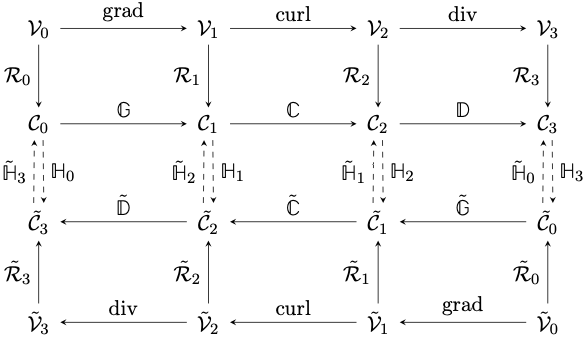
\includegraphics[width=130mm]{deRhamCGL.png}
       \caption{3D de Rham diagram}% Captions are necessary for references to work
       \label{fig:CGL_again}
    \end{figure}

    \item
    table labels should be of the form
    \verb|{tab:*}|
    \begin{table}[htbp]
          \caption{Table example \label{tab:tableEx}}
       \centering\begin{tabular}{c|c|c}
          Bread & Topping 1 & Topping 2 \\ \hline
          Rye & ham & mayonnaise\\
          Corn & ice cream & ketchup\\
       \end{tabular}
    \end{table}

\end{itemize}


\subsection{Using Box Environments in LaTeX Documentation Files}
\label{sec:boxes_in_latex}

The following box environments can be used to highlight sections:
\begin{note}
   \verb|\begin{note} \end{note}|
\end{note}
\begin{warning}
   \verb|\begin{warning} \end{warning}|
\end{warning}
\begin{error}
   \verb|\begin{error} \end{error}|
\end{error}


\end{document}
